\documentclass[dvipsnames,crop=true]{standalone}
\usepackage{tikz}
\usetikzlibrary{calc,external,3d}
\begin{document}

  \tikzsetnextfilename{layer_ec}

  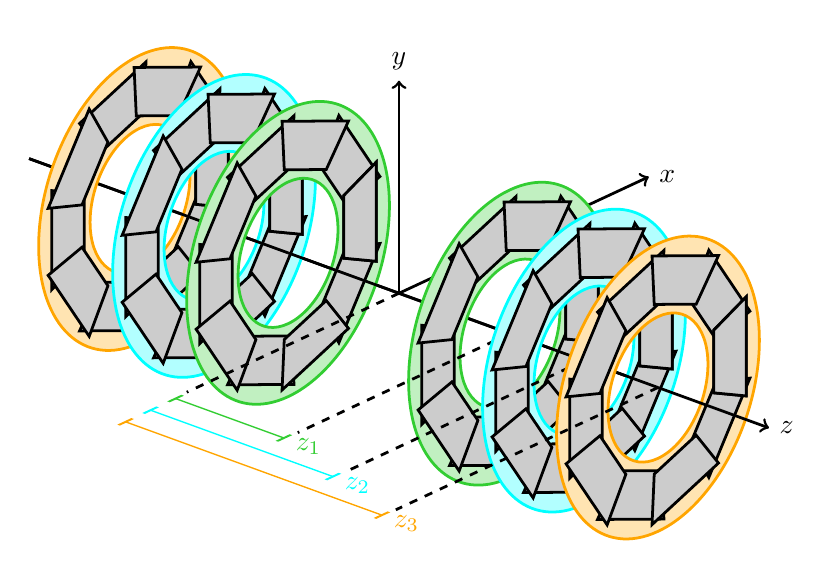
\begin{tikzpicture}[scale=1,line width=1pt]

  \def\xl{0.7cm}
  \def\yl{0.9cm}
  \def\zl{1cm}
  \def\x{({cos(25)*\xl},{sin(25)*\xl})}
  \def\y{({cos(90)*\yl},{sin(90)*\yl})}
  \def\z{({cos(-20)*\zl}, {sin(-20)*\zl})}

  % \def\xl{1cm}
  % \def\yl{1cm}
  % \def\zl{0cm}
  % \def\x{({cos(0)*\xl},{sin(0)*\xl})}
  % \def\y{({cos(90)*\yl},{sin(90)*\yl})}
  % \def\z{({cos(0)*\zl}, {sin(0)*\zl})}

  \begin{scope}[scale=1,x={(\x)},y={(\y)},z={(\z)}]
    \draw[->] (0,0,0) -- (5,0,0) node[at end,above,right] {$x$};
    \draw[->] (0,0,0) -- (0,3,0) node[at end,above] {$y$};
    \draw[-] (0,0,-5) -- (0,0,3.5);

    \coordinate(c0) at (0,0,-5);


    \def\n{10}
    \def\r{2}
    \pgfmathsetmacro{\ro}{\r+0.03}
    \pgfmathsetmacro{\ri}{\r-1}
    \def\dr{0.8}
    \pgfmathsetmacro{\da}{360/\n * 1}

    \foreach \z/\c [count=\j] in {%
      -3.5/Orange,%
      -2.5/Cyan,%
      -1.5/LimeGreen,%
      1.5/LimeGreen,%
      2.5/Cyan,%
      3.5/Orange%
      } {

      \coordinate (c\j) at (0,0,\z);

      \pgfmathsetmacro{\k}{int(\j-1)}
      \draw[] (c\k) -- (c\j);


      \begin{scope}[canvas is xy plane at z={\z}]
        % \draw[\c,fill=\c!60!white,fill opacity=0.9] (0,0) circle(\r);
        \fill[\c!30!white, even odd rule] (0,0) circle({\ro}) (0,0) circle({\ri});
        \draw[\c] (0,0) circle({\ri}) (0,0) circle({\ro});

        \foreach \i in {0,...,\n} {
          \pgfmathsetmacro{\al}{\i * \da - \da/2 * 1.2}
          \pgfmathsetmacro{\ar}{\i * \da + \da/2 * 1.2}

          \ifodd\i
            \draw[fill=black!20] (\al:{\r-\dr}) -- (\al:{\r-0.1}) -- (\ar:{\r-0.1}) -- (\ar:{\r-\dr}) -- cycle;
          \fi
        }

        \foreach \i in {0,...,\n} {
          \pgfmathsetmacro{\al}{\i * \da - \da/2 * 1.2}
          \pgfmathsetmacro{\ar}{\i * \da + \da/2 * 1.2}

          \ifodd\i
          \else
            \draw[fill=black!20] (\al:{\r-\dr}) -- (\al:{\r-0.1}) -- (\ar:{\r-0.1}) -- (\ar:{\r-\dr}) -- cycle;
          \fi
        }

        \pgfmathsetmacro{\zi}{int(\z)}
        \pgfmathsetmacro{\o}{-\zi*0.5 - 4}
        \ifnum \zi>0
          \draw [dashed,shorten >=5pt] (0,0) -- (\o,0);
        \fi

      \end{scope}
    }

    \draw[->] (0,0,3.5) -- (0,0,5) node[at end,right] {$z$};


    \begin{scope}[canvas is xz plane at y=0]
      \draw [dashed,black!100,shorten >=5pt] (0,0) -- (-4.5,0);
      \foreach \l/\c [count=\i] in {1.5/LimeGreen, 2.5/Cyan, 3.5/Orange} {
        \pgfmathsetmacro{\o}{-\i*0.5 - 4}
        % \draw [dashed,shorten <=5pt] (\o,\l) -- (0,\l);
        \begin{scope}
          \pgflowlevelsynccm
          \draw [|-|,\c,transform shape] (\o,0) --++ (0,\l);
        \end{scope}
        \node[anchor=west,shift={(0,-3pt)},\c] at (\o,\l) {$z_\i$};
      }
    \end{scope}

  \end{scope}


  \end{tikzpicture}

\end{document}